\section{ARP4761: Wheel Brake System}

\mike{Move the generic description to a section right after the ``safety'' section along with the ARP figure.  Leave the modeling that we did in AADL here.  That way we can reference it in the MBSA sections.}

As a preliminary case study, we utilized the Wheel Brake System described in ARP 4761 - Appendix L \cite{AIR6110}. The informal wheel brake system diagram is shown in Figure~\ref{fig:wbs_diagram} and is taken from the ARP 4761 document. The Wheel Brake System is installed on the two main landing gears and is used during taxi, landing, and rejected take off. Braking is either commanded manually using brake pedals or automatically with no need for the pedals (autobrake). When the wheels have traction, the autobrake function will provide a constant smooth deceleration. \\

%%%%%%%%%%%% Try to get a better figure here... this one is all blurry...
\begin{figure}[htb]
\begin{center}
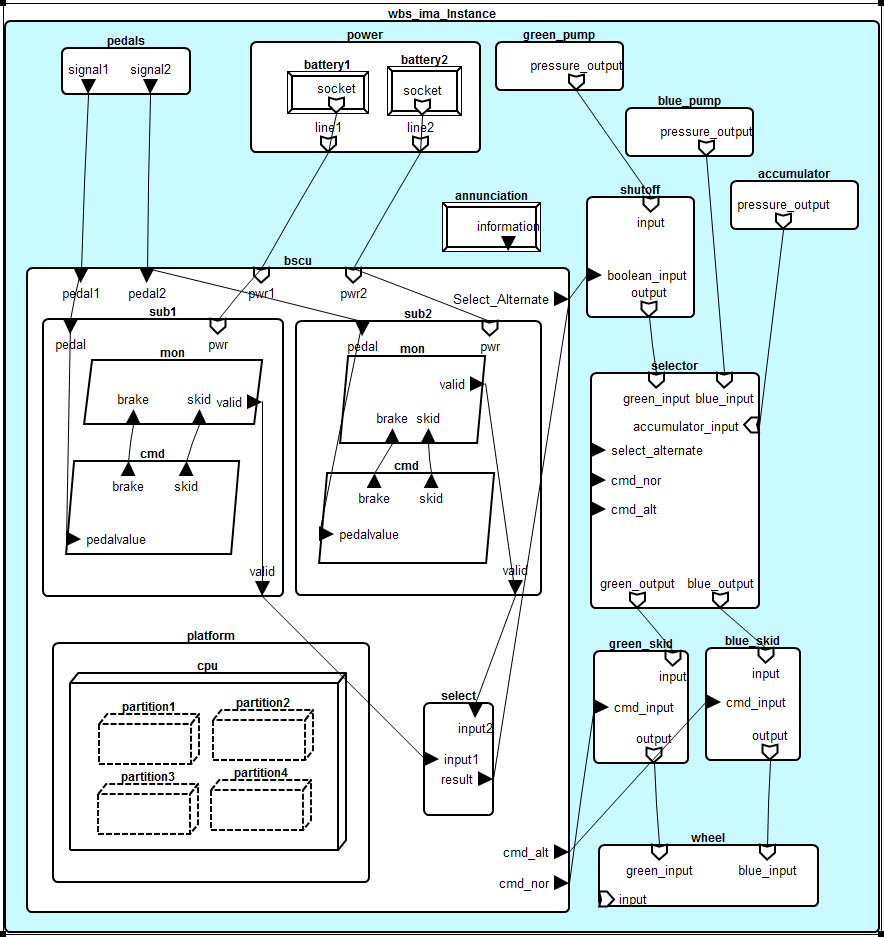
\includegraphics[scale=.75]{images/Wbs-ima}
\caption{WBS model diagram from Simple Version ARP4761 }\label{fig:wbs_diagram}
\end{center}
\end{figure}

Each wheel has a brake assembly that is operated by two sets of hydraulic pistons which operate independently. One set is operated by the Green hydraulic line which is used in NORMAL braking mode. The second system (Alternate) is operated by the Blue hydraulic line which is used when the Normal system fails. The Alternate system is also supplied by an Accumulator which is a device with built up pressure that can be released if both of the two primary pumps (Blue and Green) fail. The accumulator supplies the Alternate system in case of EMERGENCY braking mode.

Switching between the hydraulic pistons and sources can be done automatically or manually. If the normal pressure (Green) is below a certain threshold, there is an automatic switchover to the Blue supply. If the Blue pump fails, then the Accumulator is used for hydraulic pressure.

In both NORMAL and ALTERNATE modes, an anti-skid capability is available. In the Normal mode, the brake pedal position is electronically fed to a braking computer called the Braking System Control Unit (BSCU). The BSCU monitors signals that denote critical aircraft and system states to provide correct braking function, detect anomalies, broadcast warnings, and sent maintenance information to other systems.

\subsection{Nominal System Modeling}
\mike{KEEP HERE!}
A formal specification of the nominal system model consists of mechanical and digital components and their interconnections.

The highest level component is the Wheel Braking System (WBS). It consists of a digital control unit, the BSCU, and Normal and Alternate hydraulic pressure lines (supplied by Green Pump and Blue Pump/Accumulator respectively). The system takes inputs from the environment including PedalPos1, AutoBrake, DecRate, AC\_Speed, and Skid. All of these inputs are forwarded to the BSCU to compute the brake commands. The outputs of the WBS are Normal\_Pressure, Alternate\_Pressure, and System\_Mode (NORMAL, ALTERNATE, EMERGENCY).

\subsection{Braking System Control Unit (BSCU)}
The BSCU is the digital component in the system that receives inputs from the WBS. It also receives feedback from the Normal and Alternate lines and two power inputs from two separate power sources.





